\chapter{実装の詳細}

\section{ゲーム環境の実装}
2048は状態からafterstateへの遷移において, 各行~(列)~の変化は独立に考えることができる.
また回転と反転を考慮することで上下左右は等価な盤面変化を起こす.
よって$1$行の全パターンについて, ある一方向を選択したときの遷移先を前もって計算することで, 全方向に対する盤面全体の遷移を高速に行える.

\section{完全解析の実装}
回転・反転に関して同じ盤面は$1$つの状態として扱った.
またそれぞれの状態は$64$ビット整数で表現された.

$3\times3$盤面の2048の完全解析は状態列挙, 価値計算

\section{強化学習の実装}
\subsection{ニューラルネットワークの詳細}
ニューラルネットワークは盤面の特徴量を入力として, 方策と価値を出力する.
盤面サイズ$H \times W$のルールの下では理論上の最高到達タイルは$2^{H \times W + 1}$である.
このとき入力は空きマス$H \times W + 2$チャネルの$H \times W$から成る.
$n$番目のチャネルの$(i,j)$成分には盤面の$(i,j)$
\begin{figure}[t]
    \centering
    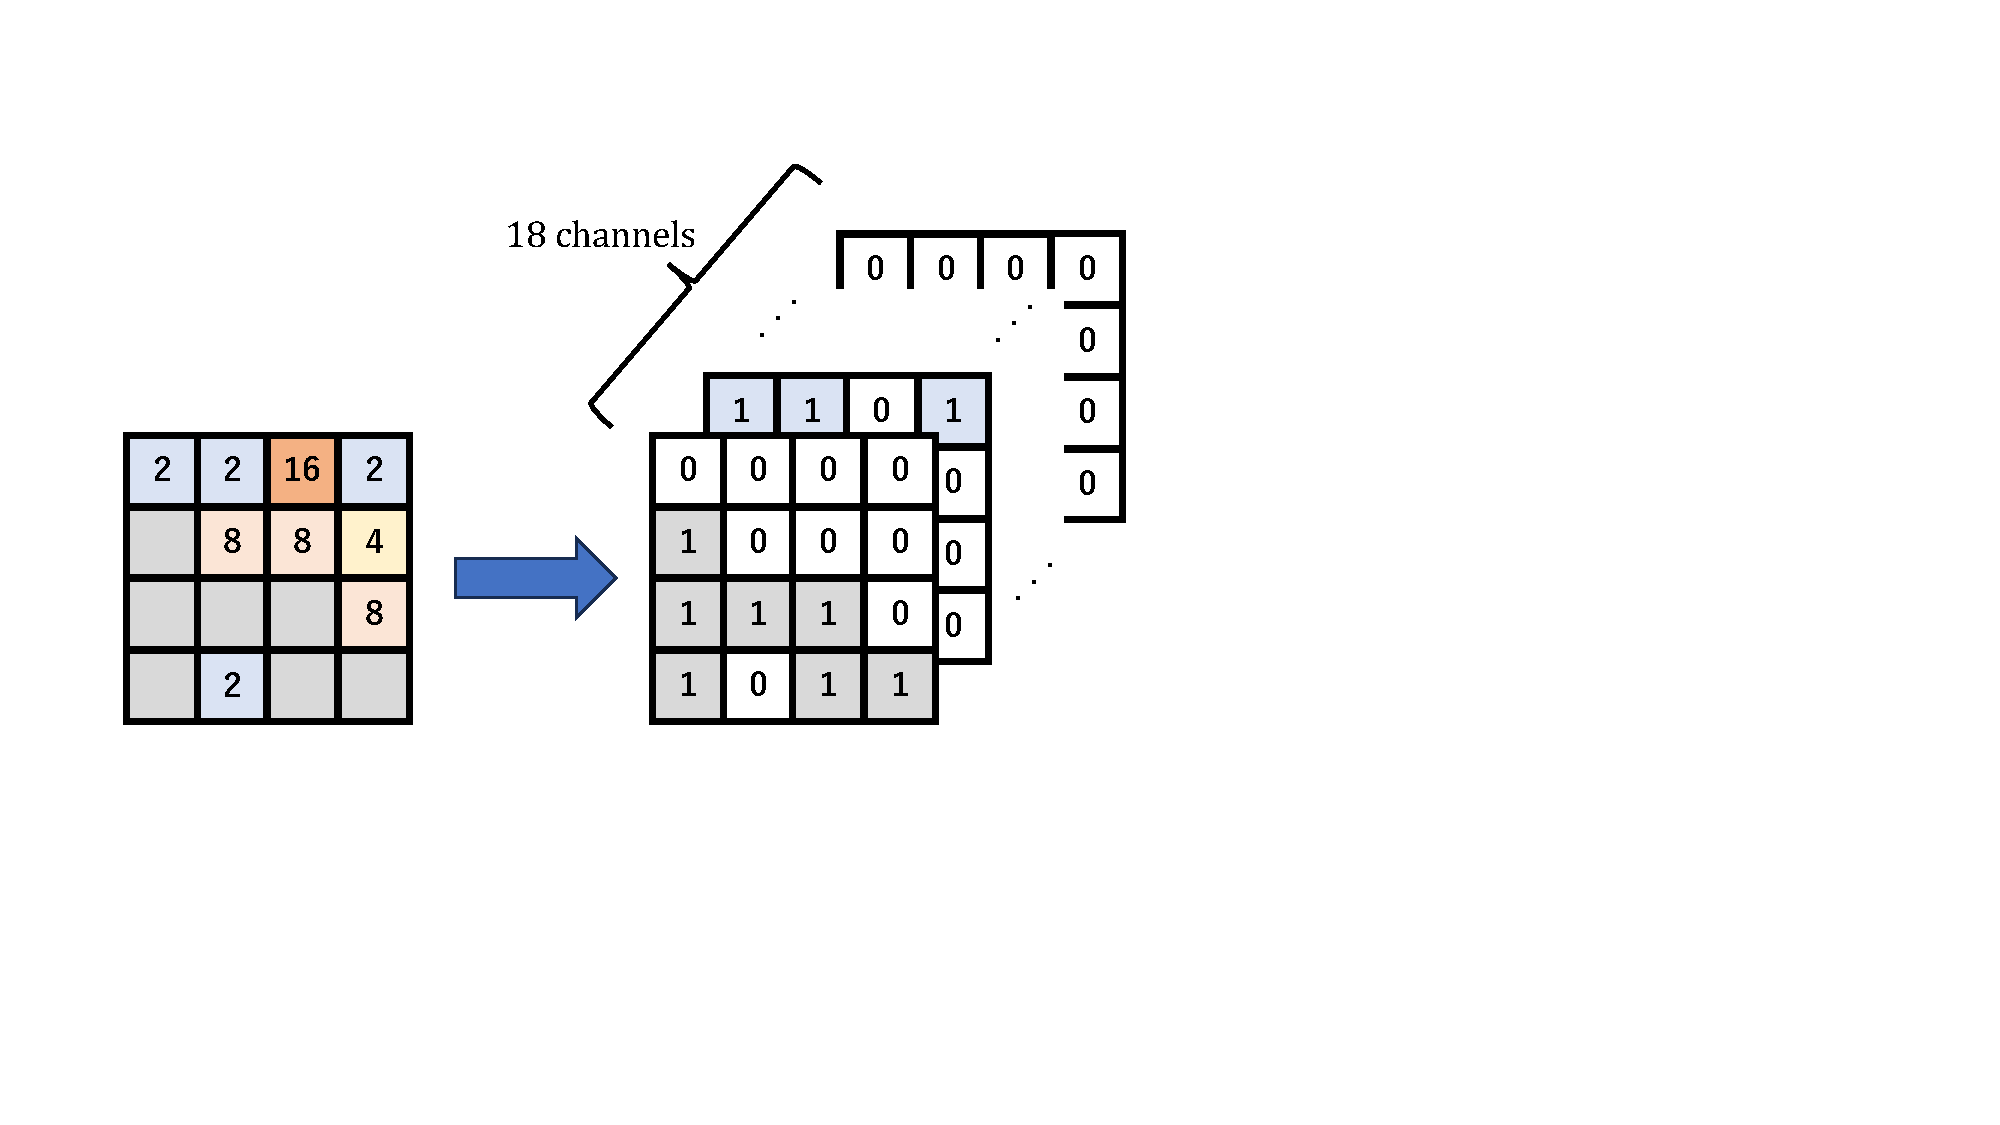
\includegraphics[width=0.6\linewidth{}]{figures/encoding.pdf}
    \caption{ニューラルネットワークへの入力特徴量}
    \label{fig:input_encoding}
\end{figure}

\subsection{Prioritized Experience Replayの詳細}
Prioritized Experience Replay~\cite{prioritized}は学習に使用するデータをランダムではなく, ある重みに従ってサンプルする手法である.
この重みをpriorityと呼び, $i$番目のデータのpriorityは$P(i) = \frac{p_{i}^{\alpha}}{\Sigma_k p_{k}^{\alpha}}$と計算される.
sum treeという二分木でデータを管理することで, $\mathcal{O}(\log n)$に改善することができる.
\begin{figure}[t]
    \centering
    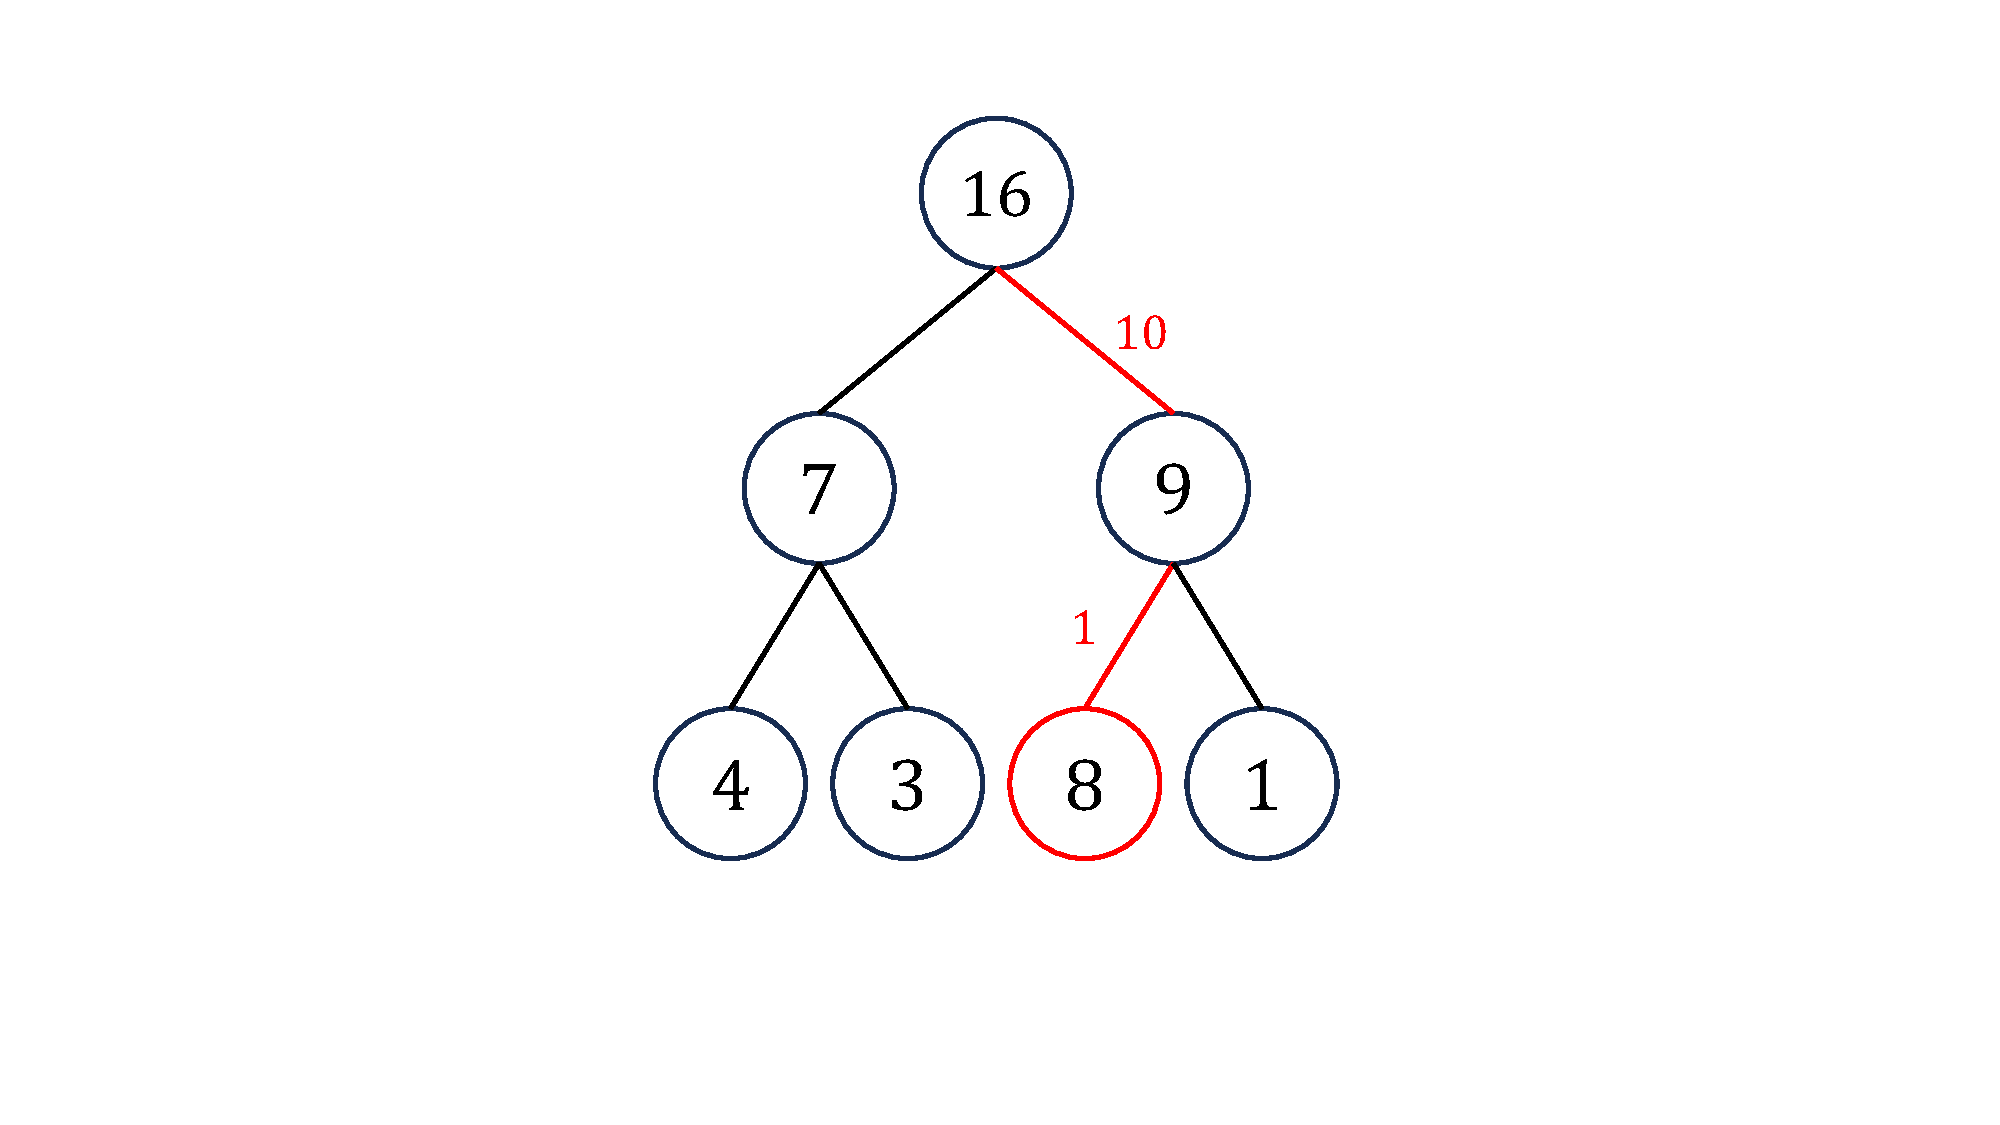
\includegraphics[width=0.6\linewidth{}]{figures/sumtree.pdf}
    \caption{sum treeの例}
    \label{fig:sumtree}
\end{figure}

\chapter{環境が“いじわる”をするルールの2048}